\documentclass[12pt,letterpaper]{exam}
\usepackage[lmargin=1in,rmargin=1in,tmargin=1in,bmargin=1in]{geometry}
\usepackage{../style/exams}

% -------------------
% Course & Exam Information
% -------------------
\newcommand{\course}{MAT 101: Exam 1}
\newcommand{\term}{Spring -- 2022}
\newcommand{\examdate}{03/10/2022}
\newcommand{\timelimit}{85 Minutes}

\setbool{hideans}{true} % Student: True; Instructor: False

% -------------------
% Content
% -------------------
\begin{document}

\examtitle
\instructions{Write your name on the appropriate line on the exam cover sheet. This exam contains \numpages\ pages (including this cover page) and \numquestions\ questions. Check that you have every page of the exam. Answer the questions in the spaces provided on the question sheets. Be sure to answer every part of each question and show all your work.} 
\scores
%\bottomline
\newpage

% ---------
% Questions
% ---------
\begin{questions}

% Question 1
\question[10] Mark each  of the following statements as True ($T$) or False ($F$). \pspace
\begin{enumerate}[(a)]
\item \underline{\hspace{1.5cm}}: $4^{100} + 4^{100} + 4^{100} + 4^{100}= 4^{101}$. \vfill
\item \underline{\hspace{1.5cm}}: The number 1 is a multiple of 12. \vfill
\item \underline{\hspace{1.5cm}}: The number 4 has three divisors. \vfill
\item \underline{\hspace{1.5cm}}: The number 1 is prime. \vfill
\item \underline{\hspace{1.5cm}}: Every integer greater than 1 is a product of prime numbers. \vfill
\item \underline{\hspace{1.5cm}}: For all real numbers $x$, we know $x^0= 1$. \vfill
\item \underline{\hspace{1.5cm}}: There is no rational number equal to $\pi$. \vfill
\item \underline{\hspace{1.5cm}}: The number $31.2 \cdot 10^5$ is in scientific notation. \vfill
\item \underline{\hspace{1.5cm}}: Two lines with positive slopes can never be perpendicular. \vfill
\item \underline{\hspace{1.5cm}}: The line $y= x + 6$ is parallel to the line $y= 7 - x$. \vfill
\end{enumerate}



\newpage



% Question 2
\question[8] Find the prime factorization for each of the following integers: \pspace
        \begin{enumerate}[(a)]
        \item $126$ \vfill
        \item $37$ \vfill
        \item $120$ \vfill
        \item $141$ \vfill
        \end{enumerate}



\newpage



% Question 3
\question[8] Compute the following: \pspace
        \begin{enumerate}[(a)]
        \item $\gcd(28, 70)$ \vfill
        \item $\lcm(28, 70)$ \vfill
        \item $\gcd(2^{500} \cdot 3^{98} \cdot 11^{82} \cdot 53^{17},\, 2^{200} \cdot 3^{50} \cdot 7^{60} \cdot 13^{300})$ \vfill
        \item $\lcm(2^{500} \cdot 3^{98} \cdot 11^{82} \cdot 53^{17},\, 2^{200} \cdot 3^{50} \cdot 7^{60} \cdot 13^{300})$ \vfill
        \end{enumerate}



\newpage



% Question 4
\question[8] Showing all your work and simplifying as much as possible, compute the following: \pspace
	\begin{enumerate}[(a)]
	\item $\dfrac{5}{12} - \dfrac{3}{4}$ \vfill
	\item $\dfrac{11}{6} + \dfrac{4}{15}$ \vfill
	\item $\dfrac{12}{55} \cdot \dfrac{5}{6}$ \vfill
	\item $\dfrac{\;\;\dfrac{20}{21}\;\;}{\dfrac{8}{7}}$ \vfill
	\end{enumerate}



\newpage



% Question 5
\question[8] Showing all your work and being sure to use no negative powers, simplify the following as much as possible: \pspace
	\begin{enumerate}[(a)]
	\item $\left( \dfrac{x^3 (x^2y^5)^0}{y^7} \right)^{-2}$ \vfill
	\item $\dfrac{(x^2 y^3)^3}{x^{10} y^{-5}}$ \vfill
	\item $(\sqrt{x^5}\, y^{-3})^4$ \vfill
	\item $\left( \dfrac{x^6}{y^5} \right)^{-1/3}$ \vfill
	\end{enumerate}



\newpage



% Question 6
\question[8] Simplify the following radical expressions: \pspace
	\begin{enumerate}[(a)]
	\item $\sqrt{36}$ \vfill
	\item $\sqrt[3]{64}$ \vfill
	\item $\sqrt{2^5 \cdot 3^2 \cdot 5}$ \vfill
	\item $\sqrt[4]{2^3 \cdot 3^9 \cdot 5^4}$ \vfill
	\end{enumerate}



\newpage



% Question 7
\question[6] Showing all your work and simplifying as much as possible, rationalize the following: \pspace
	\begin{enumerate}[(a)]
	\item $\dfrac{4}{\sqrt{6}}$ \vfill
	\item $\dfrac{1}{\sqrt[3]{7}}$ \vfill
	\item $\dfrac{1}{3 - \sqrt{5}}$ \vfill
	\end{enumerate}



\newpage



% Question 8
\question[8] Showing all your work, convert 5~km/s$^2$ to miles per square minute. Note that 1~km $=$ 1000~m, 1~ft $=$ 0.3048~m, and 60~s $=$ 1~min.



\newpage



% Question 9
\question[4] Complete the following:
	\begin{enumerate}[(a)]
	\item Convert the following number in scientific notation to an ordinary \par decimal number: $-4.73 \cdot 10^{-6}$ \vfill
	\item Convert the following ordinary decimal number to scientific notation: $0.054$ \vfill
	\end{enumerate} \vfill

% Question 10
\question[8] Showing all your work, compute the following: \pspace
        \begin{enumerate}[(a)]
        \item 97 decreased by 60\% \vfill
        \item 573 increased by 142\% \vfill
        \item 71\% of 140 \vfill
        \end{enumerate}



\newpage



% Question 11
\question[8] Compute the following, being sure to show all your work and to write your answer in the form $a + bi$: \pspace
	\begin{enumerate}[(a)]
	\item $(3i)^3$ \vfill
	\item $(6 + 4i) - (4 - 4i)$ \vfill
	\item $(1 + i)(3 - 2i)$ \vfill
	\item $\dfrac{6 + i}{1 - i}$ \vfill
	\end{enumerate}



\newpage



% Question 12
\question[8] Suppose a student has a 90\% participation average, 75\% quiz average, 84\% homework average, 86\% on the midterm, and 66\% on the final exam, given that their course grade is computed using the weights below, find their course average:
	\begin{table}[!ht]
	\centering
	\begin{tabular}{rr}
	Participation: & 5\% \\
	Quizzes: & 15\% \\
	Homework: & 45\% \\
	Midterm: & 15\% \\
	Final: & 20\%
	\end{tabular}
	\end{table}



\newpage



% Question 13
\question[8] Answer the following:
	\[
	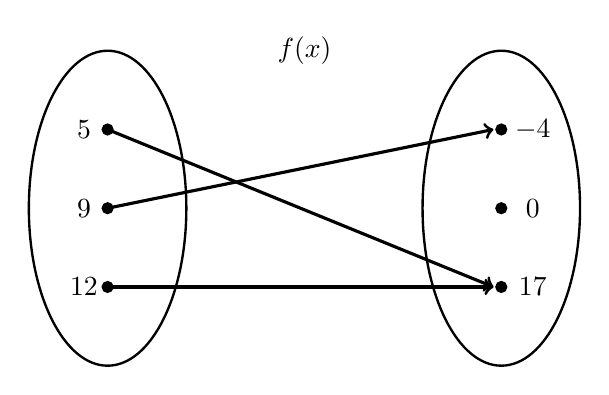
\begin{tikzpicture}
	\node at (2.5,2) {$f(x)$};
	% Ellipses
	\draw[line width=0.03cm] (0,0) circle (1 and 2);
	\draw[line width=0.03cm] (5,0) circle (1 and 2);
	
	% Nodes
	\draw[fill=black] (0,1) circle (0.07);
	\draw[fill=black] (0,0) circle (0.07);
	\draw[fill=black] (0,-1) circle (0.07);
	
	\draw[fill=black] (5,1) circle (0.07);
	\draw[fill=black] (5,0) circle (0.07);
	\draw[fill=black] (5,-1) circle (0.07);
	
	% Arrow
	\draw[line width=0.04cm,->] (0,1) -- (4.9,-1);
	\draw[line width=0.04cm,->] (0,0) -- (4.9,1);
	\draw[line width=0.04cm,->] (0,-1) -- (4.9,-1);
	
	% Labels
	\node at (-0.3,1) {$5$};
	\node at (-0.3,0) {$9$};
	\node at (-0.3,-1) {$12$};
	
	\node at (5.4,1) {$-4$};
	\node at (5.4,0) {$0$};
	\node at (5.4,-1) {$17$};
	\end{tikzpicture}
	\] \pspace

\begin{enumerate}[(a)]
\item Explain why the relation $f(x)$ above is a function. \vfill
\item Find the domain, codomain, and range of the function $f(x)$. \vfill
\item Is the relation $g(x)= 17x - x^3$ a function? Explain. \vfill
\end{enumerate}



\newpage



% Question 14
\question[8] Consider the relation $f(x)$ plotted below.
	\[
	\fbox{
	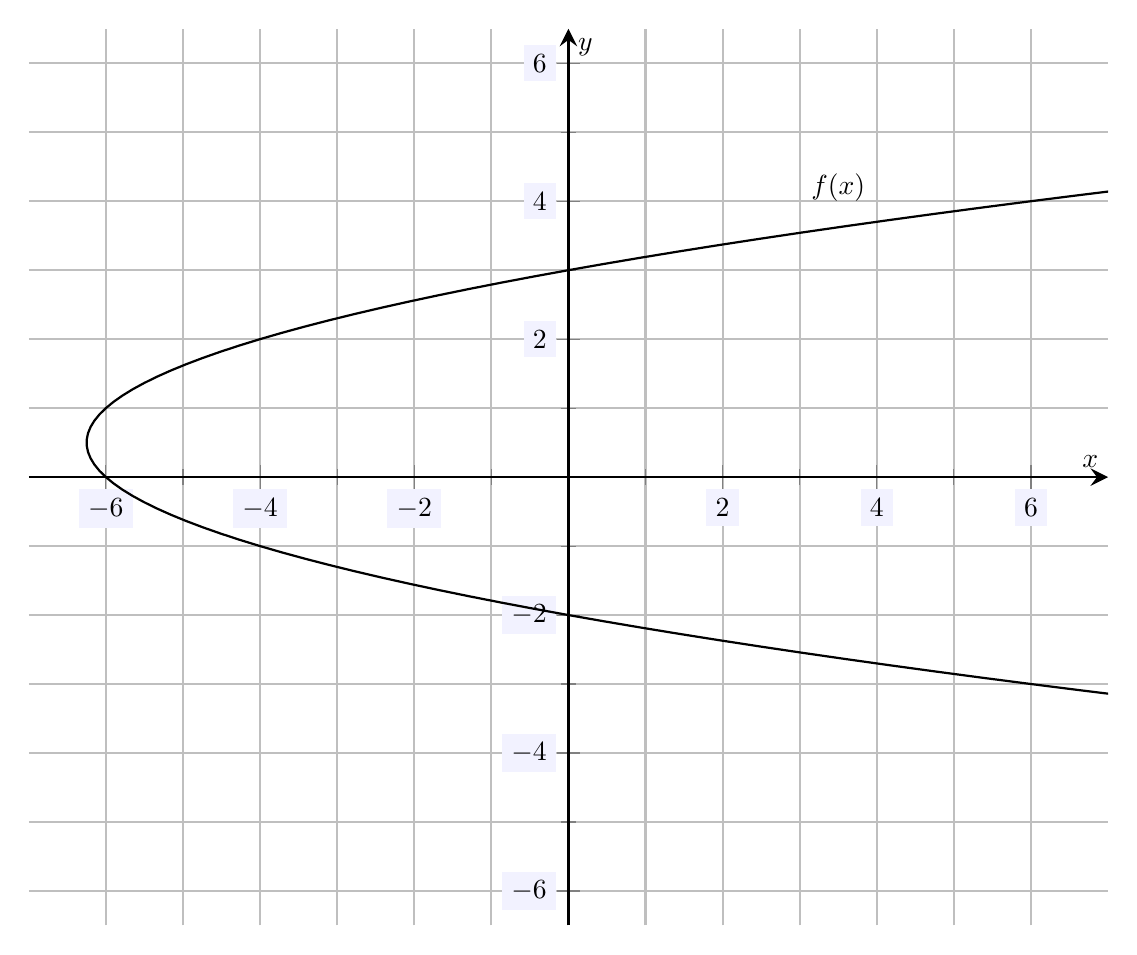
\begin{tikzpicture}[scale=2,every node/.style={scale=0.5}]
	\begin{axis}[
	grid=both,
	axis lines=middle,
	ticklabel style={fill=blue!5!white},
	xmin= -7, xmax=7,
	ymin= -6.5, ymax=6.5,
	xtick={-6,-4,-2,0,2,4,6},
	ytick={-6,-4,-2,0,2,4,6},
	minor tick = {-5,-3,...,5},
	xlabel=\(x\),ylabel=\(y\),
	]
	\node at (3.5,4.2) {$f(x)$};
	\addplot [domain= -4:5,samples=100] ({x^2 - x - 6},{x}); 
	\end{axis}
	\end{tikzpicture}
	}
	\] \pspace

\begin{enumerate}[(a)]
\item Is the relation $f(x)$ plotted above a function? Explain. \vfill
\item Does the relation above have an inverse function? Explain. \vfill
\item Find the $y$-intercepts of the relation plotted above. \vfill
\item Find the $x$-intercepts of the relation plotted above. \vfill
\end{enumerate}



\newpage



% Question 15
\question[6] Consider the functions given in the table below.
        \begin{table}[!ht]
        \centering
        \begin{tabular}{| c || r | r | r | r | r |} \hline
	$x$ & $-2$ & $-1$ & $0$ & $1$ & $2$ \\ \hline
	$f(x)$ & $5$ & $-2$ & $-5$ & $-3$ & $2$ \\ \hline
	$g(x)$ & $6$ & $2$ & $10$ & $7$ & $-5$ \\ \hline
        \end{tabular}
        \end{table}

Compute the following: \pspace
        \begin{enumerate}[(a)]
        \item $g(2)=$ \vfill
        \item $(f - g)(0)=$ \vfill
        \item $(fg)(1)=$ \vfill
        \item $\left( \dfrac{g}{f} \right)(0)=$ \vfill
        \item $(f \circ g)(-1)=$ \vfill
        \item $(g \circ f)(-1)=$ \vfill
        \end{enumerate}



\newpage



% Question 16
\question[8] Consider the function $\ell(x)= 6 - 2x$. \pspace
	\begin{enumerate}[(a)]
	\item Is $\ell(x)$ linear? Explain. \vfill
	\item Find the slope of $\ell(x)$. \vfill
	\item Find the $y$-intercept of $\ell(x)$. \vfill
	\item Is the point $(-1, 4)$ on the graph of $\ell(x)$? Explain. \pvspace{3cm}\vfill
	\end{enumerate}



\newpage



% Question 17
\question[6] Find the equation of the line perpendicular to $y= 6 - 2x$ at its $x$-intercept. 



\newpage



% Question 18 
\question[6] Solve the following equation and then verify your solution:
	\[
	3x -14= 8 - \frac{2}{3}\,x
	\]


\newpage



% Question 19
\question[8] You are driving home from university at 55~mph. Your home is 650~miles from your university. Assuming you left the university 2~hours ago and that you drive at a constant speed, find your distance from your home, $D(t)$, as function of time $t$, in hours. 



\newpage



% Question 20
\question[8] You rent an apartment in NYC, which you paid a \$50 application fee to apply for. The rent is \$2500/month. Therefore, the amount you have paid, $R(t)$, to rent the apartment $t$ months after moving in is given by $R(t)= 2500t + 50$.
	\begin{enumerate}[(a)]
	\item Without knowing $R(t)$, how do you know that $R(t)$ is linear? \vfill
	\item What is the slope of $R(t)$ and what does it represent in the problem context? \vfill
	\item What is the $y$-intercept of $R(t)$ and what does it represent in the problem context? \vfill
	\end{enumerate}

\end{questions}
\end{document}